\subsection{Modeling Job Dependencies}

The overall goal of the FAUST framework is to schedule a given set of jobs on a number of distributed resources as effective as possible. Effectiveness in our case means minimum \textit{makespan}\footnote{The makespan of a schedule is its total execution time.} scheduling or time to completion. In case of an application which consists of a
set of independent jobs (embarrassingly parallel EP), scheduling is rather trivial:
execute as many jobs as possible at the same time on all available resources. An
example for such an application would be a parameter sweep which generates and executes  a set of independent model instances with different input parameters.

However, lots of distributed applications do not fall into the category of EP applications. Jobs often require communication with other jobs or they may rely on data  that has to be generated by other jobs. Message-passing (e.g. MPI) as well as distributed workflows are good examples for these types of applications. Unfortunately, scheduling becomes way more complex in this case, since it has to take not only the availability of resources but also things like interconnect bandwidth, shared filesystems, etc. into account to minimize the overhead exposed by job dependencies.

In this section, we try to identify different types of job dependencies, describe how to model them on application level and discuss the implications for possible minimum 
makespan scheduling algorithms.

\subsubsection{Types of Dependencies}

So far, we identified two types of dependencies in distributed applications that are relevant for job scheduling and placement. We distinguish between dependencies that rely on data availability and dependencies that rely on communication:


\textbf{Data Dependencies} occur whenever a job requires data that is generated by another job or a set of jobs. Imagine an image processing application (Figure \ref{fig:data_dependencies}) that splits up an image into several regions and applies a filter to each of the regions in parallel. Another job takes the processed fragments and puts them back together. This job depends on the output generated by the filter instances. 

    \begin{figure}[bth!]
    \begin{center}
      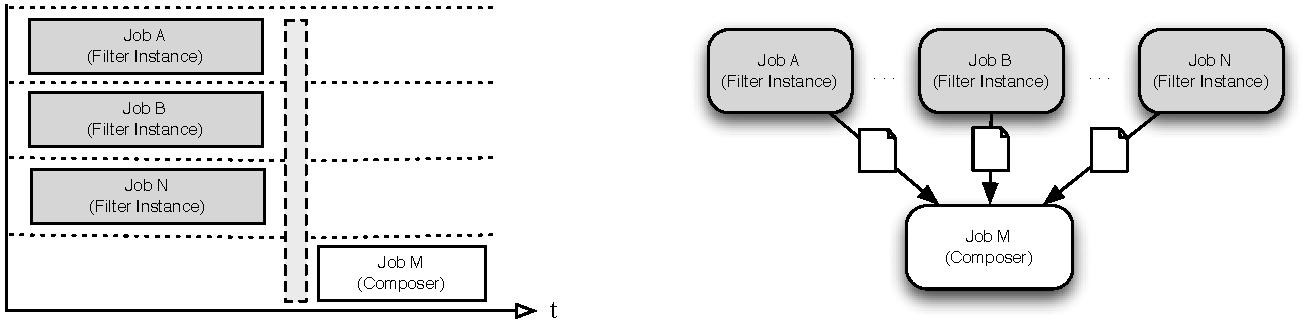
\includegraphics[width=0.95\textwidth]{figures/data_dependencies}
      \caption{\label{fig:data_dependencies} Example of a dependency graph \textit{(r)} for an image processing application where job \textit{M} depends on the data generated by jobs \textit{A...N}. The grey vertical bar in the scheduling scheme \textit{(l)} represents the time overhead generated by data transfer.}
    \end{center}
  \end{figure}


\textbf{Communication Dependencies} occur whenever two or more jobs need to exchange information while they are running. Imagine a 2D heat-tansfer application (Figure \ref{fig:comm_dependencies}) that splits up the problem space in 4 regions and maps them to 4 different jobs (domain decomposition). Communication has to occur whenever the heat transfers across domain boundaries. This concept is also known as ghost-zone exchange and a very well known concept in MPI.

    \begin{figure}[h]
    \begin{center}
      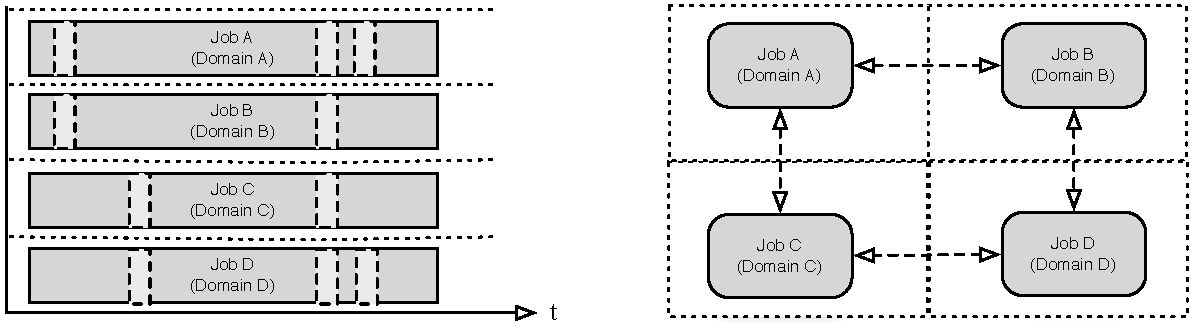
\includegraphics[width=0.95\textwidth]{figures/comm_dependencies}
      \caption{\label{fig:comm_dependencies} Example of a dependency graph \textit{(r)} for set of communicating jobs in a domain decomposition application. The grey vertical bars within the jobs in the scheduling scheme \textit{(l)} represent the time overhead generated by communication.}
    \end{center}
  \end{figure}

\subsubsection{Describing Dependencies}

Describing just the dependencies and type of dependencies (data or communication) between jobs enables a scheduler to execute the 
jobs in a way that satisfies the dependencies. However, without additional information about the jobs and the dependencies, a scheduling algorithm won't be able to \textit{place} the jobs efficiently. These attributes usually can't be extracted from the application automatically. They have to be described explicitly on application level. We identify a minimum set of these attributes and show how they can be described using the FAUST API.

\textbf{Data Dependencies} expose a potential data transfer overhead. A scheduling algorithm has to decide wether it should either move the data to the computation or the computation to the data (place the dependent job as close\footnote{\textit{Close} in this context is defined as the interconnect bandwidth between two locations.} to the data as possible). To be able to make this decision, the following information has to be provided on application level:

\begin{itemize}
\item \textbf{Expected runtime} of the jobs that are part of the dependency. \begin{verbatim}faust::attribute::walltime\end{verbatim}
\item \textbf{Expected amount of data} generated by a job.
\begin{verbatim}faust::attribute::data_volume\end{verbatim}
\end{itemize}

The FAUST framework provides an interface to describe data dependencies in applications through the \textit{job submission} interface. In case of the example image processing application described above, this could look like the following (simplified) code fragment:

 \begin{mycode}[label=Describing Data Dependencies]
 
    job::description filter_jd;
    filter_jd.set_attribute(walltime, "10.0");
    filter_jd.set_attribute(data_volume, "0.5GB");
    
    std::vector<std::string> filter_desc;
    for(int i=1; i<10; ++i)
      filter_desc.push_back(filter_jd); // create 10 filter instances
    
    job::service s;
    job::group filters = s.create_job_group(filter_desc);

    // create the composer job which has a DATA dependency with the
    // filter job group. 
    job::description composer_jd;
    job::job composer = s.create_job(composer_jd, filters, type::DATA);
    
    s.schedule();
  
 \end{mycode}

\textbf{Communication Dependencies} expose a potential communication overhead. A scheduling algorithm has to decide... The following application attributes can help a scheduling algorithm to make this decision:

\begin{itemize}
\item Compute/communication ratio
\item Type of communication (TCP/UDP/...) 
\end{itemize}
